\documentclass[specialist,
               substylefile = ../spbu.rtx,
               subf,href,colorlinks=true, 12pt]{disser}

\usepackage[a4paper,
            mag=1000, includefoot,
            left=3cm, right=1.5cm, top=2cm, bottom=2cm, headsep=1cm, footskip=1cm]{geometry}
\usepackage[T2A]{fontenc}
\usepackage[utf8]{inputenc}
\usepackage[english,russian]{babel}

\let\bibfont\relax
\usepackage{biblatex}
\addbibresource{../biblio-u.bib}

\ifpdf\usepackage{epstopdf}\fi

% Точка с запятой в качестве разделителя между номерами цитирований
%\setcitestyle{semicolon}

% Использовать полужирное начертание для векторов
% \let\vec=\mathbf

% Включать подсекции в оглавление
\setcounter{tocdepth}{2}

\usepackage{graphicx}
\graphicspath{ {../media/} }

\usepackage[intlimits]{amsmath}
\usepackage{amsfonts}
\usepackage{amssymb}
\usepackage{amsthm}

\usepackage{hyperref}
\newtheorem{theorem}{Теорема}
\newcommand{\E}{\mathrm{E}}
\newcommand{\vfi}{\varphi}
\newcommand{\eps}{\varepsilon}
\newcommand{\prob}[1]{\mathrm{P}\left(#1\right)}
\newcommand{\R}{\ensuremath{\mathbb{R}}}
\newcommand{\Tau}{\ensuremath{\mathcal{T}}}
\newcommand{\GothB}{\mathfrak{B}}
\newcommand{\norm}[1]{\left\lVert#1\right\rVert}
\newcommand{\abs}[1]{\left\lvert#1\right\rvert}
\newcommand{\Vhat}{\hat{V}}
\newcommand{\vhat}{\hat{v}}
\newcommand{\maxset}[1]{\max\left\lbrace#1\right\rbrace}
\newcommand{\deltat}{\Delta t}
\DeclareMathOperator{\correlation}{cor}
\newcommand{\corr}[2]{\correlation\left(#1, #2\right)}
\DeclareMathOperator*{\argmax}{arg\,max}
\DeclareMathOperator*{\argmin}{arg\,min}
\DeclareMathOperator{\dd}{d}

% \usepackage[fixlanguage]{babelbib}
% \selectbiblanguage{russian}
% \setbtxfallbacklanguage{russian}


%----------------------------------------------------------------
\begin{document}

%
% Титульный лист на русском языке
%

% Название организации
\institution{%
    Санкт-Петербургский государственный университет \\
    Прикладная математика и информатика \\
    Статистическое моделирование
}

\title{Отчет о научно-исследовательской работе}

% Тема
\topic{\normalfont\scshape%
    Методы оценки Американского опциона}

% Автор
\author{Миллер Анастасия Александровна}

% Научный руководитель
\sa       {С.\,М.~Ермаков}
\sastatus {д.\,ф.-м.\,н., профессор}

% Город и год
\city{Санкт-Петербург}
\date{\number\year}

\begin{large}
\maketitle
\end{large}

\tableofcontents

\intro
В работе рассмотрены основные подходы к оценке стоимости Американских опционов и приведено их сравнение между собой (как теоретическое, так и на численных примерах). Приведены некоторые методы снижения дисперсии: классические метод противоположных переменных и метод контрольных переменные и более редко используемый метод рандомизированного квази Монте-Карло.

Основной вопрос, исследованный в этом семестре --- применение метода квази Монте-Карло к оценкам и сравнение его с основными методами снижения дисперсии (глава \ref{cha:quasi_monte_carlo}).

В главе \ref{cha:option_price_estimation_problem} описана задача оценки Американских опционов (в секции \ref{sec:option_price}) и приведены основные методы её решения (случайные деревья, стохастические сетки и линейная регрессия, раздел \ref{sec:estimators}). 
% Глава \ref{cha:variance_reduction} содержит описание методов снижения дисперсии оценок, в частности, применение квази Монте-Карло. 
В главе \ref{cha:quasi_monte_carlo} более подробно разобрана теория квази Монте-Карло и приведены обоснования для выбора размерности квазислучайной последовательности. %В большинстве секций теоретические сведения подкреплены демонстрацией вычислений на конкретных примерах.

\chapter{Задача оценки стоимости Американского опциона} % (fold)
\label{cha:option_price_estimation_problem}

Опцион --- это широко распространённый вторичный (производный) финансовый инструмент. Опцион является контрактом между продавцом опциона и покупателем опциона о том, что покупатель имеет право, но не обязательство, купить (в случае опциона на покупку, call option) или продать (в случае опциона на продажу, put option) указанный в контракте базовый актив по заранее оговорённой цене в определённый контрактом момент в будущем или на протяжении определённого отрезка времени. Продавца опциона контракт обязует совершить ответную продажу (для опциона на покупку) или покупку (для опциона на продажу) в случае, если покупатель пожелает исполнить своё право. Реализация такой сделки называется \emph{исполнением опциона}.

Различают опционы европейского и американского типа. Опцион европейского типа выписывается на фиксированный момент времени в будущем, опцион американского типа --- на отрезок времени. Промежуточный вариант, когда опцион может быть исполнен только в определённые даты (например, в конце каждого квартала в течение года), часто называют Бермудским опционом.

Исполнение опциона может быть выгодно его владельцу (когда цена базового актива в контракте ниже текущей рыночной в случае опциона на покупку, когда цена базового актива выше текущей рыночной в случае опциона на продаже), поэтому опционный контракт сам по себе тоже имеет стоимость. Ищется стоимость опциона в модели эффективного рынка, то есть такая цена, при которой ни продавец, ни покупатель опциона в среднем не получают прибыли.

\section{Стоимость Американского опциона как случайная величина} % (fold)
\label{sec:option_price}

В случае опциона европейского типа существует решение в замкнутой форме (модель Блэка-Шоулса \cite{Black1973} и её усовершенствования). Оценка Американского опциона является более сложной задачей.

Опцион определяется своим временем жизни $[0;T]$, базовым активом $X$ (под $X(t)$ будем подразумевать состояние актива в момент времени $t$, являющееся случайной величиной, $S(t) = S(X(t))$ --- цену базового актива в момент $t$), на который выписан опцион (список возможных активов на территории Российской Федерации представлен в \cite{fsfr}), процессом $U(t), t\in [0;T]$, представляющим дисконтированное значение функции выплат (разницы между рыночной стоимостью базового актива и ценой страйк, оговорённой в контракте; значение функции выплат показывает выгоду, получаемую владельцем опциона при исполнении), и множеством $\Tau$ моментов времени, в которых возможно исполнить опцион. Будем также считать, что существует $h_t: U(t) = h_t\left(X(t)\right)$. Тогда для Американского опциона с функцией выплат $h_t\left(X_t\right)$, задача оптимального исполнения --- это задача о нахождении 
\begin{equation}\label{eq:optimal_stopping}
V = \max_{\tau} \E h_\tau\left(X_\tau\right).
\end{equation}

При дискретизации \eqref{eq:optimal_stopping} (принятии предположения о том, что опцион может быть исполнен только в некотором конечном числе моментов времени $\left\lbrace t_i\right\rbrace_{i=0}^n \in \left[0;T\right], t_0 = 0, t_n = T$) задача обретает эквивалентную формулировку о нахождении $V_0\left(X_0\right)$ для
\begin{equation}\label{eq:option-recursive}\begin{aligned}
			V_m\left(x\right) &= h_m\left(x\right), \\
			V_{i-1}\left(x\right) &= \max\left\lbrace h_{i-1}\left(x\right), \E\left[V_i\left(X_i\right)|X_{i-1}=x\right]\right\rbrace.
\end{aligned}\end{equation}

% section option_price (end)

\section{Оценки} % (fold)
\label{sec:estimators}

Наверное, самый простой способ оценить стоимость Американского опциона --- это промоделировать много вариантов траекторий базового актива, посчитать выплату по опциону в каждом случае и усреднить результаты. Это классический метод Монте-Карло.

Все предложенные ниже способы --- это различные попытки уменьшить дисперсию наивного варианта путём увеличения числа моделируемых траекторий. 

\subsection{Случайные деревья} % (fold)
\label{sub:tree_estimator}

Метод случайного дерева основан на моделировании цепи $X_0, X_1, \ldots X_n$ состояний актива. Зафиксируем параметр ветвления $b$. Из исходного состояния $X_0$ смоделируем $b$ независимых следующих состояний $X_1^1, X_1^2, \ldots X_1^b$, все с условием $X_0$. Для каждого $X_1^i$ снова смоделируем $b$ независимых последующих состояний $X_2^{i1}, \ldots X_2^{ib}$. На $m$-ом шаге будем иметь $b^m$ состояний, и это и есть источник основного недостатка этого метода --- его экспоненциальной алгоритмической сложности. Схема приведена на рис. \ref{fig:exponential_tree}.
\begin{figure}[h]
    \centering
	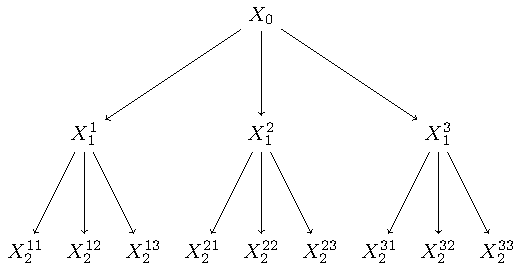
\includegraphics{exponential_tree.pdf}
	\caption{Случайное дерево для $b = 3$ и $m = 2$}
	\label{fig:exponential_tree}
\end{figure}

В \cite{Broadie1997} предложены оценки сверху и снизу $\hat{V}_0$ и $\hat{v}_0$ и доказана их состоятельность и асимптотическая несмещённость для $V_0\left(S_0\right)$.
\begin{align}\label{eq:upper}
	\hat{V}_m^{j_1 \ldots j_m} &= h_m\left(S_m^{j_1 \ldots j_m}\right), \\
	\hat{V}_i^{j_1 \ldots j_i} &= \max \left\lbrace h_i \left( S_i^{j_1 \ldots j_i} \right), \frac{1}{b} \sum_{j = 1}^b \hat{V}_{i+1}^{j_1 \ldots j_i j}\right\rbrace,
\end{align}
\begin{align}\label{eq:lower}
	\hat{v}_m^{j_1 j_2 \cdots j_m} &= h\left( S_m^{j_1 j_2 \cdots j_m}\right), \\
	\hat{v}_{ik}^{j_1 j_2 \cdots j_i} &= \left\lbrace
			    \begin{array}{l l}
				    h\left( S_i^{j_1 j_2 \cdots j_i}\right), & \, \text{если } \frac{1}{b-1}\sum_{j=1, j\not= k}^b \hat{v}_{i+1}^{j_1 j_2 \cdots j_i j} \leq h\left(S_i^{j_1 j_2 \cdots j_i}\right), \\
				    \hat{v}_{i+1}^{j_1 j_2 \cdots j_i k}, & \, \text{иначе}
			    \end{array}\right. \\
	\hat{v}_i^{j_1 j_2 \cdots j_i} &= \frac{1}{b}\sum_{k=1}^b \hat{v}_{ik}^{j_1 j_2 \cdots j_i}.
\end{align}

Алгоритм прост в реализации и нетребователен по памяти: при реализации обходом в глубину память ограничена $O(m)$. Основной недостаток -- экспоненциальная сложность по времени: обойти всё дерево получится за $O(m^b)$.

% subsection tree_estimator (end)

\subsection{Стохастические сетки} % (fold)
\label{sub:mesh_estimator}

Метод стохастической сетки также предлагает оценки сверху и снизу для решения \eqref{eq:option-recursive}, но принцип построения оценок несколько отличается от рассматриваемых мною оценок по случайному дереву.

Из начального состояния $X_0$ для оценки опциона с $m$ моментами исполнения, равноотстоящими во времени от 0 до $T$, зададим сетку $X_n^i, n\in 1\mathbin{:}m, i \in 1\mathbin{:}b$, узлы которой --- реализации случайной величины с плотностью $p_{0, n}(X_0, \cdot)$ (маргинальные плотности; также рассматриваются средние плотности), а $p_{k, n}(x, y) = \prob{X_n = y \middle\vert X_k = x}$. Тогда определяется $\rho_{n, j}(x, y) = p_{n-1, n}(x, y) / p_{0, n}(X_0, y)$, сокращённые обозначения $\rho_{n, j}(i, j) = \rho_{n, j}(X_{n-1}^i, X_n^j)$ и оценка в каждом узле сетки
$$\hat Y_n(i) = \max\left\lbrace h_n(i), \frac{\sum_j \rho_{n+1}(i, j) \hat Y_{n+1}(j)}{\sum_j \rho_{n+1}(i, j)} \right\rbrace.$$

Иллюстрация взаимоотношений между узлами сетки приведена на рис.~\ref{fig:stochastic_mesh}. Тогда оценка справедливой стоимости опциона --- это $$\hat Y_0 = \max\left\lbrace h_0(X_0), \frac{\sum_j \rho_{1}(X_0, X_1^j) \hat Y_{1}(X_1^j)}{\sum_j \rho_{1}(X_0, X_1^j)} \right\rbrace.$$

\begin{figure}[h]
    \centering
	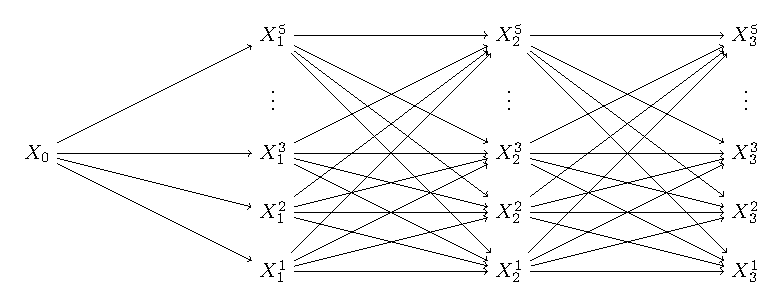
\includegraphics{stohastic_mesh_vector.eps}
	\caption{Стохастическая сеть для $b = 5$ и $m = 3$}
	\label{fig:stochastic_mesh}
\end{figure}

Этот метод работает гораздо быстрее, чем метод случайных деревьев: сложность и по времени, и по памяти составляет $O(mb)$. Недостатком являются трудоёмкие вычисления в многомерном случае: в отличие от случайного дерева, для обсчёта которого нужно лишь уметь вычислить $h_t(X_t)$ (для традиционного примера максимум-опциона на покупку $h_t(X_t) = \left(\max(X_t) - K\right)^+$, если $X_t$ -- вектор стоимостей базовых активов в момент $t$), для стохастических сетей нужно точно вычислять $\rho_n(i, j)$.

% subsection mesh_estimator (end)

\subsection{Метод наименьших квадратов} % (fold)
\label{sub:least_squares}

Несколько отличающийся от двух предыдущих вариант --- метод оценки с помощью линейной регрессии. Согласно формулировке \eqref{eq:option-recursive}, в каждый момент $t$ мы хотим знать математическое ожидание стоимости удержания (неисполнения) опциона при условии его текущего состояния. Классический инструмент для оценки условного математического ожидания --- это линейная регрессия. Будем оценкивать стоимость удержания опциона следующим образом:

$$\E\left(V_i(X_i)\middle\vert X_{i-1} = x\right) \approx \sum_{r=1}^M \beta_{ir} \psi_r(x) = \beta_i^\mathsf{T}\psi(x).$$

Здесь $\psi(x) = \left(\psi_1(x), \dots, \psi_M(x)\right)$ --- это набор регрессоров, используемых для построения оценки. В оригинальной статье \cite{Longstaff2001} использовались полиномы Лагера (секция~2.2 на стр.~122).

\begin{figure}[h]
    \centering
	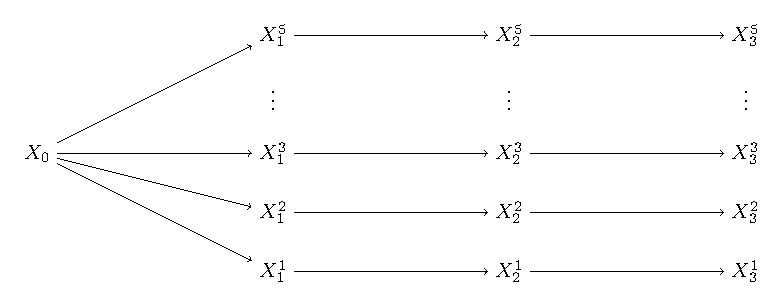
\includegraphics{stohastic_mesh_vector_phase_0.eps}
	\caption{Стохастическая сеть для $b = 5$ и $m = 3$}
	\label{fig:least_squares}
\end{figure}

Мы используем сетку, аналогичную той, что была в методе стохастической сетки: моделируем несколько траекторий, тем самым получая нужный набор примеров (см. рис.~\ref{fig:least_squares}). Коэффициенты $\beta$ оцениваются по методу наименьших квадратов. В результате мы получаем следующий алгоритм оценки:

\begin{equation}
	\begin{aligned}
	\Vhat_m^j &= h_m(X_m^j), \quad \hat\beta_i = \argmin_{\beta\in\R^m} \norm{\left(\beta^\mathsf{T}\psi(X_i^j) - \Vhat_{i+1}^j\right)_{j=1}^b}^2 \\
		\Vhat_i^j &= \maxset{h_i(X_i^j), \hat \beta_i^\mathsf{T}\psi(x)},\;\; \Vhat_0 = \frac{1}{b}\sum_{j=1}^b V_1^j\end{aligned}\label{eq:least_squares}
\end{equation}

В \cite{Glasserman2004} указано, что метод наименьших квадратов можно считать частным случаем метода стохастической сетки со специальным выбором весов. Тем не менее, часто эти подходы рассматриваются по отдельности.

% subsection least_squares (end)

% section estimators (end)

% % chapter option_price_estimation_problem (end)

% \chapter{Методы снижения дисперсии} % (fold)
% \label{cha:variance_reduction}

% \section{Противоположные переменные} % (fold)
% \label{sec:antithetic_variables}

% % section antithetic_variables (end)

% \section{Контрольные переменные} % (fold)
% \label{sec:control_variates}

% % section control_variates (end)

% \section{Квази Монте Карло} % (fold)
% \label{sec:quasi_monte_carlo}

% % section quasi_monte_carlo (end)

% chapter variance_reduction (end)

\chapter{Квази Монте Карло} % (fold)
\label{cha:quasi_monte_carlo}

\section{Основные понятия} % (fold)
\label{sec:quasi_mc_definition}

Отклонением (star discrepancy, $D^*$) последовательности из $N$ $d$-мерных случайных векторов в гиперкубе $\left[0;1\right]^d$ называют величину
$$D_N^* = D_N^*\left(X_1, \dots, X_N\right) = \sup_{v = (v_1, \dots, v_d) \in \left[0;1\right]^d} N \abs{\frac{\#\left\{ X_i \in J(v) \right\}}{N} - \prod_{j = 1}^d v_j},$$
где $J(v) = \left[0; v_1\right) \times \dots \times \left[0; v_d\right)$.

В случае, когда последовательность $\left\{ X_i\right\}_{i=1}^\infty$ такова, что $\forall N \: D_N^* \leq C_s \frac{(\ln N)^s}{N}$, последовательность называется последовательностью с низким отклонением (или с низким дискрепансом). С вычислительной точки зрения она представляет интерес из-за неравенства Коксмы-Хлавки: для интеграла, оцененного по этой последовательности, верно утверждение

$$\abs{\int_{\left[0;1\right]^d} f(X) \dd X - \frac{1}{N}\sum_{i=1}^N f(X_i)} \leq \mathrm{Var}f\cdot \frac{D_N^*\left(X_1, \dots, X_N\right)}{N},$$
где $\mathrm{Var}f$ -- вариация функции в смысле Харди-Краузе. При $N\to\infty$ эта оценка погрешности лучше, чем оценка погрешности классического Монте-Карло.
% section quasi_mc_definition (end)

\section{Приложение к задаче оценки стоимости Американского опциона} % (fold)
\label{sec:monte_carlo_in_option_pricing}

\subsection{Преобразование в нормальное распределение} % (fold)
\label{sub:uniform_normal_transform}

Квази Монте-Карло обычно рассматривается в контексте задачи интегрирования функции на $\left[0;1\right]^d$, а параллели проводятся с классическим Монте-Карло с использованием распределения $\mathrm U\left[0;1\right]^d$. В финансовых задачах же обычно используются нормальное и логнормальное распределения, но не равномерное. Поэтому первый вопрос, которому стоит уделить внимание --- это вопрос о корректном преобразовании, которое переводило бы последовательность с нихким дискрепансом на $\left[0;1\right]^d$ в последовательность с низким дискрепансом по мере нормального распределения. Согласно \cite{Oekten2011}, преобразование Бокса-Мюллера, применённое к <<распрямлённой>> квазислучайной последовательности, применимо в этом случае.

% subsection uniform_normal_transform (end)

\subsection{Выбор размерности} % (fold)
\label{sub:choice_of_dimension}

В контексте задачи многомерного интегрирования, в которой обычно говорится о квази Монте-Карло, размерность пространства, по которому происходит интегрирование, является условием задачи. В случае задачи оценивания опционов ответ на вопрос о том, какой же должна быть размерность квазислучайной последовательности, не столь очевиден.

Во-первых, если исходить из того, что функцией, математическое ожидание которой мы оцениваем, является весь обсчёт сетки или дерева, то размерность интегрируемого пространства --- это конструктивная размерность алгоритма, то есть $\sum_{i=1}^m b^i$ для оценки по случайным деревьям и $mb$ для метода сетки или наименьших квадратов.

В случае сколько-нибудь разумных $m$ и $b$ (например, $m = 3$ и $b = 50$) конструктивная размерность линейных методов уже достаточно высока для квазислучайных последовательностей, а для метода случайных деревьев гораздо выше допустимых пределов. Так, для построения последовательности Холтона размерности 150 нужно получить 150 взаимно простых чисел. В случае, когда мы берём последовательность простых чисел, 150-е из них равно 853. Это означает, что по построению последовательности последняя координата первых её 852 точек будет идти равноотстоящими шагами от 0 до 1, что уже не очень похоже на случайные равномерно распределённые на $\left[0; 1\right]$ числа, и рандомизация сдвигом не исправит ситуацию. Это известный недостаток последовательности Холтона, аналогичные проблемы с большими размерностями имеют и другие квазислучайные последовательности.

Поэтому можно использовать другой подход: взять некоторую достаточно большую размерность $n$, взять последовательность из $k$ квазислучайных чисел $\left(x_1^i, \dots, x_n^i\right)$  этой размерности, распрямить (получится вектор $\left(x_1^1, \dots, x_n^1, x_1^2, \dots, x_n^k\right)$ длины $nk$) и работать с ней как с последовательностью из обычного генератора псевдослучайных чисел.

Третий вариант --- это использование размерности, равной размерности базового актива. В конечном счёте оценка стоимости опциона является комбинацией интегралов по пространству состояний базового актива ($\E\left(V_i(X_i)\middle\vert X_{i-1} = x\right)$), и именно эти интегралы мы оцениваем.

% subsection choice_of_dimension (end)

\subsection{Численные результаты} % (fold)
\label{sub:numerical_results}

На рис.~\ref{fig:halton_estimators} приведены результаты моделирования для всех трёх вариантов, применённых к методу случайных деревьев. Вариант с конструктивной размерностью алгоритма посчитан только для $b = 10$, так как для б\'oльших значений $b$ посчитать его не представляется возможным. В таблице~\ref{tbl:halton_estimators} приведены численные значения и доверительные интервалы для оценок.

\begin{figure}[h]
    \centering
	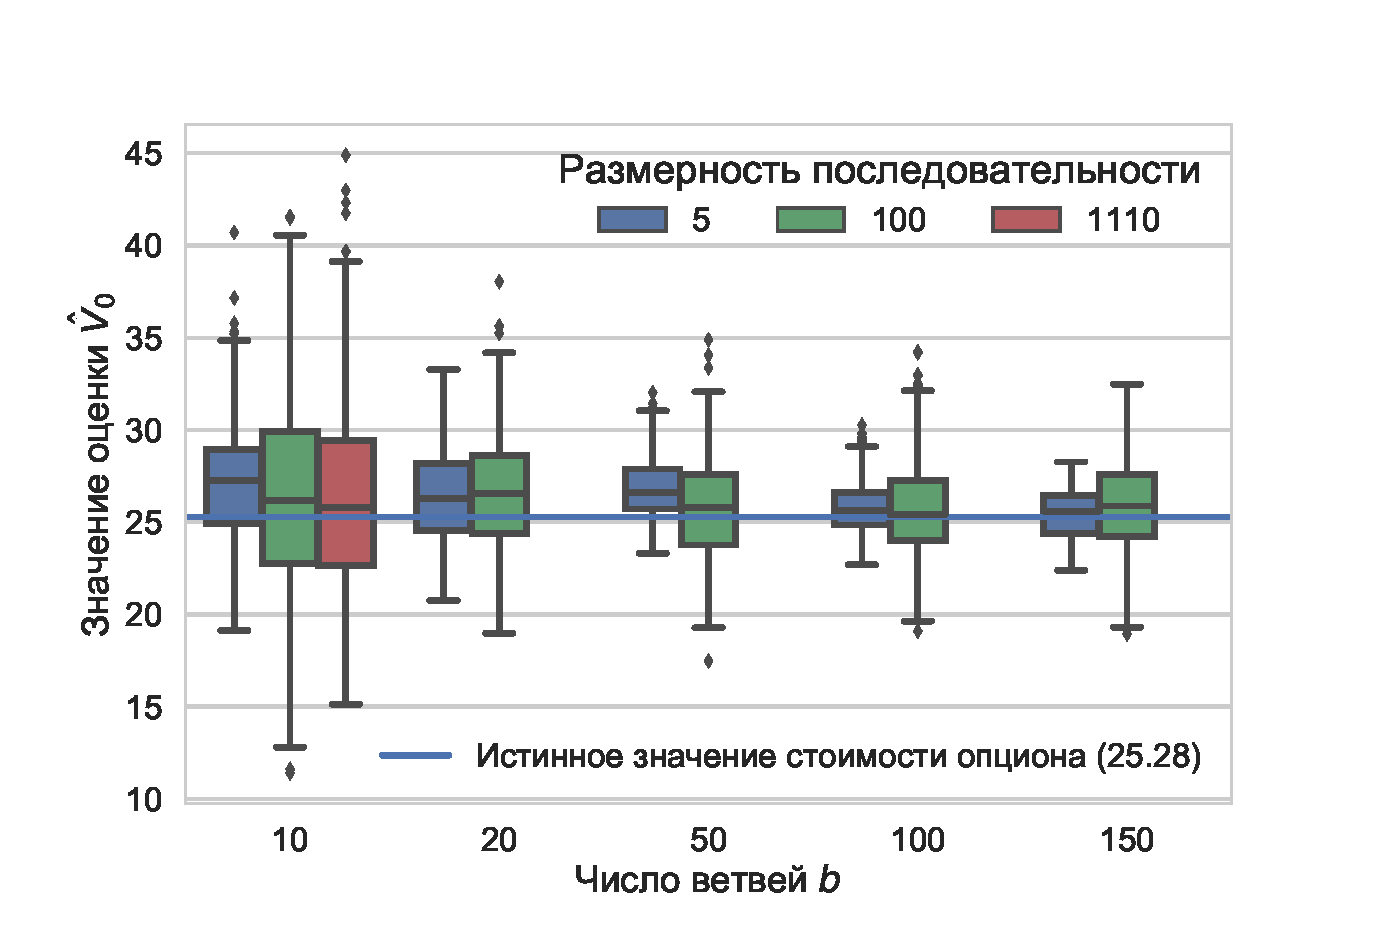
\includegraphics[width=\textwidth]{halton_estimators.eps}
	\caption{Оценки рандомизированными квазислучайными последовательностями}
	\footnotesize Опцион на 5 независимых базовых активов с $r = 5\%, \delta = 10\%, \sigma = 20\%$. Платёжная функция $h_t(X_t) = \left(\max(X_t) - K\right)^+, X_t\in \mathbb R^5$. Начальная цена каждого из активов $S_0 = 100$, цена страйк $K = 100$, опцион выписан на $T=3$ года. Опцион имеет 4 момента исполнения: в $0, T/3, 2T/3$ и $T$. Вычисления методом случайных деревьев.
	\label{fig:halton_estimators}
\end{figure}

\begin{table}
	\renewcommand{\arraystretch}{0.6}
	\centering
	\caption{Оценки, полученные с помощью рандомизированных квазислучайных последовательностей разных размерностей}
	\begin{tabular}{rrrrr}
		$b$&$d$&$\Vhat_0$&$\mathrm{sd}\Vhat_0$&доверительный интервал\\[5pt]\hline\\
		10&5&27.159&3.122&[26.929; 27.390]\\
		10&100&26.383&5.448&[25.982; 26.785]\\
		10&1110&26.34&5.037&[25.969; 26.711]\\[5pt]
		20&5&26.386&2.406&[26.209; 26.564]\\
		20&100&26.559&3.192&[26.323; 26.794]\\[5pt]
		50&5&26.839&1.568&[26.723; 26.954]\\
		50&100&25.774&2.667&[25.578; 25.971]\\[5pt]
		100&5&25.849&1.457&[25.742; 25.956]\\
		100&100&25.656&2.547&[25.468; 25.844]\\[5pt]
		150&5&25.464&1.239&[25.372; 25.555]\\
		150&100&26.016&2.413&[25.783; 26.250]\\[10pt]
	\end{tabular}
	\label{tbl:halton_estimators}

	\footnotesize
	Результаты приведены для числа ветвей $b = 10, 20, 50, 100, 150$ и размерности квазислучайной последовательности $d = 5, 100, 1110$. Колонка $\Vhat_0$ содержит усреднённое значение $\Vhat_0$ по 500 испытаниям (рандомизация последовательности Холтона при этом проходила $M = 10$ раз, каждая страта содержит 100 испытаний), в колонке $\mathrm{sd}\Vhat_0$ приведены значения стандартного отклонения.
\end{table}

Можно заметить, что разультаты с размерностью 5 имеют значительно меньшую дисперсию, чем результаты с размерностью 100. Предположительно это объясняется приведёнными выше соображениями о нерегулярности сетки при использовании больших размерностей.

Сравнение рандомизированного квази Монте-Карло (варианта с последовательностями размерности, равной размерности базового актива) с классическим Монте-Карло приведено на рис.~\ref{fig:quasi_vs_common_mc}. Дисперсия оценки с использованием рандомизированного квази Монте-Карло выглядит меньше, чем дисперсия обычного Монте-Карло. 

Для отклонений оценки от среднего была проверена гипотеза $U$-теста Манна-Уитни (верно ли, что случайно взятое отклонение от среднего оценки, вычисленной по квазислучайным числам, будет с одинаковой вероятностью больше или меньше случайно взятого отклонения от среднего оценки, вычисленной по псевдослучайной последовательности) против альтернативы о том, что отклонения оценок по квазислучайным числам меньше отклонений по псевдослучайным числам. $p$-value гипотезы равно 0.0017, так что дисперсия квази Монте-Карло статистически значимо меньше дисперсии обычного Монте-Карло в этом численном эксперименте.

\begin{figure}[h]
    \centering
	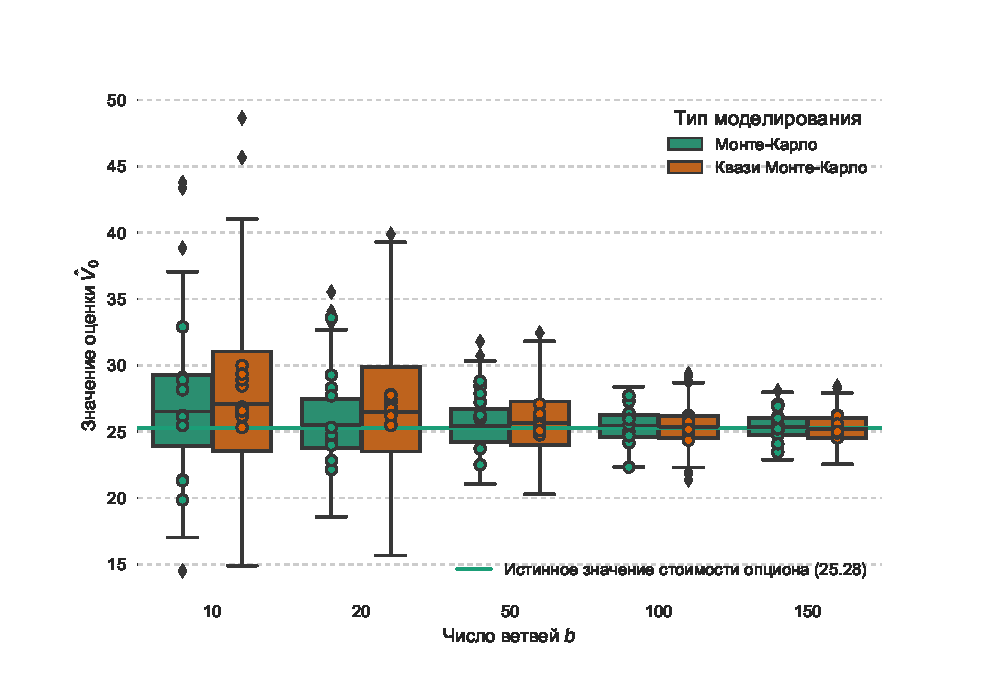
\includegraphics[width=\textwidth]{quasi_vs_common_mc.eps}
	\caption{Сравнение рандомизированной квазислучайной последовательности и стандартного метода}
	\footnotesize Опцион на 5 независимых базовых активов с $r = 5\%, \delta = 10\%, \sigma = 20\%$. Платёжная функция $h_t(X_t) = \left(\max(X_t) - K\right)^+, X_t\in \mathbb R^5$. Начальная цена каждого из активов $S_0 = 100$, цена страйк $K = 100$, опцион выписан на $T=3$ года. Опцион имеет 4 момента исполнения: в $0, T/3, 2T/3$ и $T$. Вычисления методом случайных деревьев.
	\label{fig:quasi_vs_common_mc}
\end{figure}

\begin{table}
	\renewcommand{\arraystretch}{0.6}
	\centering
	\caption{Оценки, полученные с помощью рандомизированных квазислучайных последовательностей разных размерностей}
	\begin{tabular}{rrrrr}
		$b$&тип последовательности&$\Vhat_0$&$\mathrm{sd}\Vhat_0$&доверительный интервал\\[5pt]\hline\\
		10&Квази Монте-Карло&27.159&3.122&[26.929; 27.390]\\
		10&Монте-Карло&26.691&4.149&[26.385; 26.997]\\[5pt]
		20&Квази Монте-Карло&26.386&2.406&[26.209; 26.564]\\
		20&Монте-Карло&25.69&2.746&[25.488; 25.893]\\[5pt]
		50&Квази Монте-Карло&26.839&1.568&[26.723; 26.954]\\
		50&Монте-Карло&25.499&1.832&[25.364; 25.634]\\[5pt]
		100&Квази Монте-Карло&25.849&1.457&[25.742; 25.956]\\
		100&Монте-Карло&25.419&1.164&[25.333; 25.504]\\[10pt]
	\end{tabular}
	\label{tbl:quasi_vs_common_mc}

	\footnotesize
	Результаты приведены для числа ветвей $b = 10, 20, 50, 100$ и псевдослучайных и квазислучайных последовательностей. Колонка $\Vhat_0$ содержит усреднённое значение $\Vhat_0$ по 500 испытаниям (рандомизация последовательности Холтона при этом проходила $M = 10$ раз, каждая страта содержит 100 испытаний), в колонке $\mathrm{sd}\Vhat_0$ приведены значения стандартного отклонения.
\end{table}

% subsection numerical_results (end)

% section monte_carlo_in_option_pricing (end)

% chapter quasi_monte_carlo (end)

\conclusion

В этом семестре я исследовала вопрос о применимости рандомизированных квазислучайных последовательностей к задаче оценивания Американского опциона. Полученные результаты (см.~\ref{sub:numerical_results}) показывают, что квазислучайные последовательности могут быть применены в этой задаче и дают статистически значимый прирост точности. 

Пока остался за рамками остался вопрос о комбинировании этой техники с такими приёмами уменьшения дисперсии, как противоположные переменные и контрольные переменные, но результаты исследования этого вопроса будут включены в ВКР. Ещё один важный вопрос, который нельзя оставлять без рассмотрения --- это влияние рандомизации квазислучайной последовательности на общее смещение оценки. Оценки, для которые представлены численные результаты, являются смещёнными вверх, а для парных к ним смещённых вниз вычисления пока ещё не были проведены.

Тем не менее, основной результат работы --- квазислучайные последовательности применимы и существует вполне определённая размерность такой последовательности, дающая наименьшую дисперсию --- уже получен.

\printbibliography

\end{document}

